\chapter{Cadre général}
\begin{spacing}{1.2}
\minitoc
\thispagestyle{MyStyle}
\end{spacing}
\newpage

\section*{Introduction}

\noindent Pour bien concevoir et développer notre application, nous allons présenter les différents aspects de ce projet en commençant par l'organisme d'accueil, puis la définition du projet avec ses objectifs et le travail demandé. Nous présenterons ensuite la méthodologie adoptée et la démarche suivie pour réaliser le projet.

\section{Context général du projet}

\noindent Notre projet intitulé "Prévention Plus", réalisé au sein de SWConsulting, s'inscrit dans le cadre du projet de fin d'études à l'École Supérieure Privée d'Ingénieurs de Monastir (ESPRIM) pour l'obtention du diplôme national d'ingénieur en Génie Informatique.

\subsection{Problématique}

\noindent Les bureaux de conseil en sécurité et qualité utilisent encore des processus d'audit manuels qui sont lents et sujets aux erreurs. Les entreprises demandent plus de traçabilité et de conformité aux normes, mais les solutions existantes sont soit trop générales soit trop chères pour les PME de conseil.

Comment développer une solution digitale spécialisée et accessible qui simplifie les audits tout en respectant les standards de qualité et sécurité ?

\subsection{Organisme d'accueil}

\noindent\large\textbf{Présentation de l'entreprise}\normalsize
\vspace{0.3em}

\noindent SWConsulting est une agence web basée à Monastir, Tunisie, spécialisée dans les services informatiques depuis sa création en 2016. Employant entre 11 et 50 collaborateurs, dont une équipe de 12 développeurs, l'entreprise se distingue par son expertise dans le développement de solutions numériques pour les TPE, PME et grands groupes, principalement en Europe. SWConsulting a travaillé avec divers secteurs, notamment l'assurance, les agences de voyages et le pharmaceutique, en accompagnant des clients dans la digitalisation de leurs processus.

\begin{figure}[H]%
    \center%
{
    
\includegraphics[width=5cm,height=4cm]{images/logoent.jpg}%
    }
    \caption{Logo SWConsulting}%
\end{figure}

\noindent\large\textbf{Activités de l'entreprise}\normalsize
\vspace{0.3em}

\noindent SWConsulting propose les services suivants :
\begin{itemize}
    \item \textbf{Développement web et mobile} : Création de sites e-commerce (PrestaShop), sites vitrine (WordPress, HTML5/PHP), applications web sur mesure (utilisant Zend, Laravel, Angular) et applications mobiles pour Android et iOS. L'équipe développe des solutions robustes adaptées aux besoins spécifiques des clients.

    \item \textbf{CRM et automatisation} : Conception et mise en place de systèmes CRM pour optimiser les processus métier et améliorer la gestion de la relation client.

    \item \textbf{Référencement SEO} : Optimisation du référencement naturel pour accroître la visibilité en ligne des sites web de ses clients.

    \item \textbf{Marketing digital} : Gestion de campagnes en ligne, incluant la création de bannières et l'envoi de courriels promotionnels.
\end{itemize}

\subsection{Étude de l'existant}

\noindent Après des recherches approfondies, il s'avère qu'il existe déjà des applications web pour la gestion d'audits et d'autres pour l'évaluation de conformité.

\noindent\textbf{AuditBoard}\normalsize
\vspace{0.3em}

\noindent AuditBoard [2] est une plateforme de gestion des risques et de conformité qui permet aux entreprises de gérer leurs audits internes. Elle compte plus de 6000 organisations utilisatrices dans le monde. En plus de la gestion d'audits, elle offre des modules de gestion des risques et de conformité réglementaire.

\begin{figure}[H]%
    \center%
{
    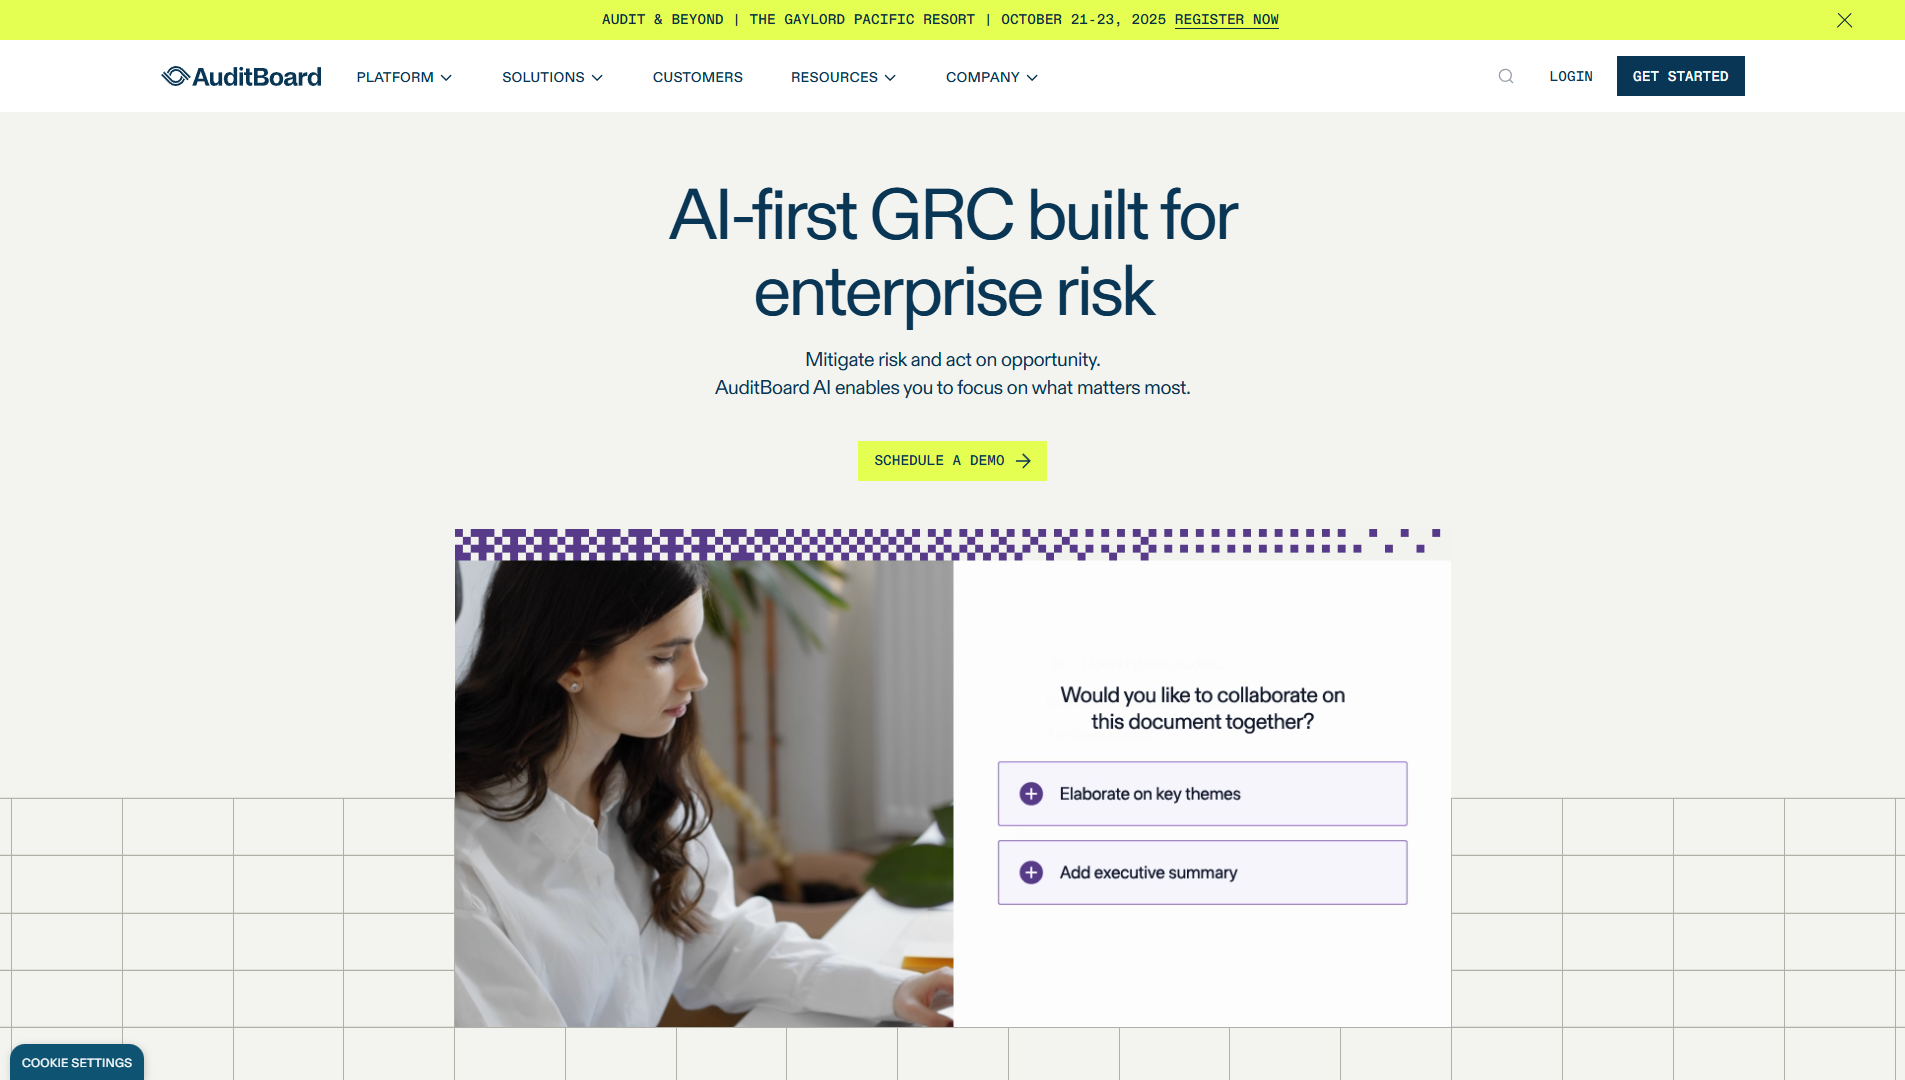
\includegraphics[width=13cm,height=8cm]{images/auditboard.PNG}%
    }
    \caption{Site web AuditBoard}%
\end{figure}

\noindent\textbf{ProcessGene}\normalsize
\vspace{0.3em}

\noindent ProcessGene [3] est une solution de gestion de la conformité et des processus métier qui permet aux organisations de créer et suivre leurs audits en ligne. Elle permet de partager les audits avec des codes d'accès privés ou des liens publics.

\begin{figure}[H]%
    \center%
{
    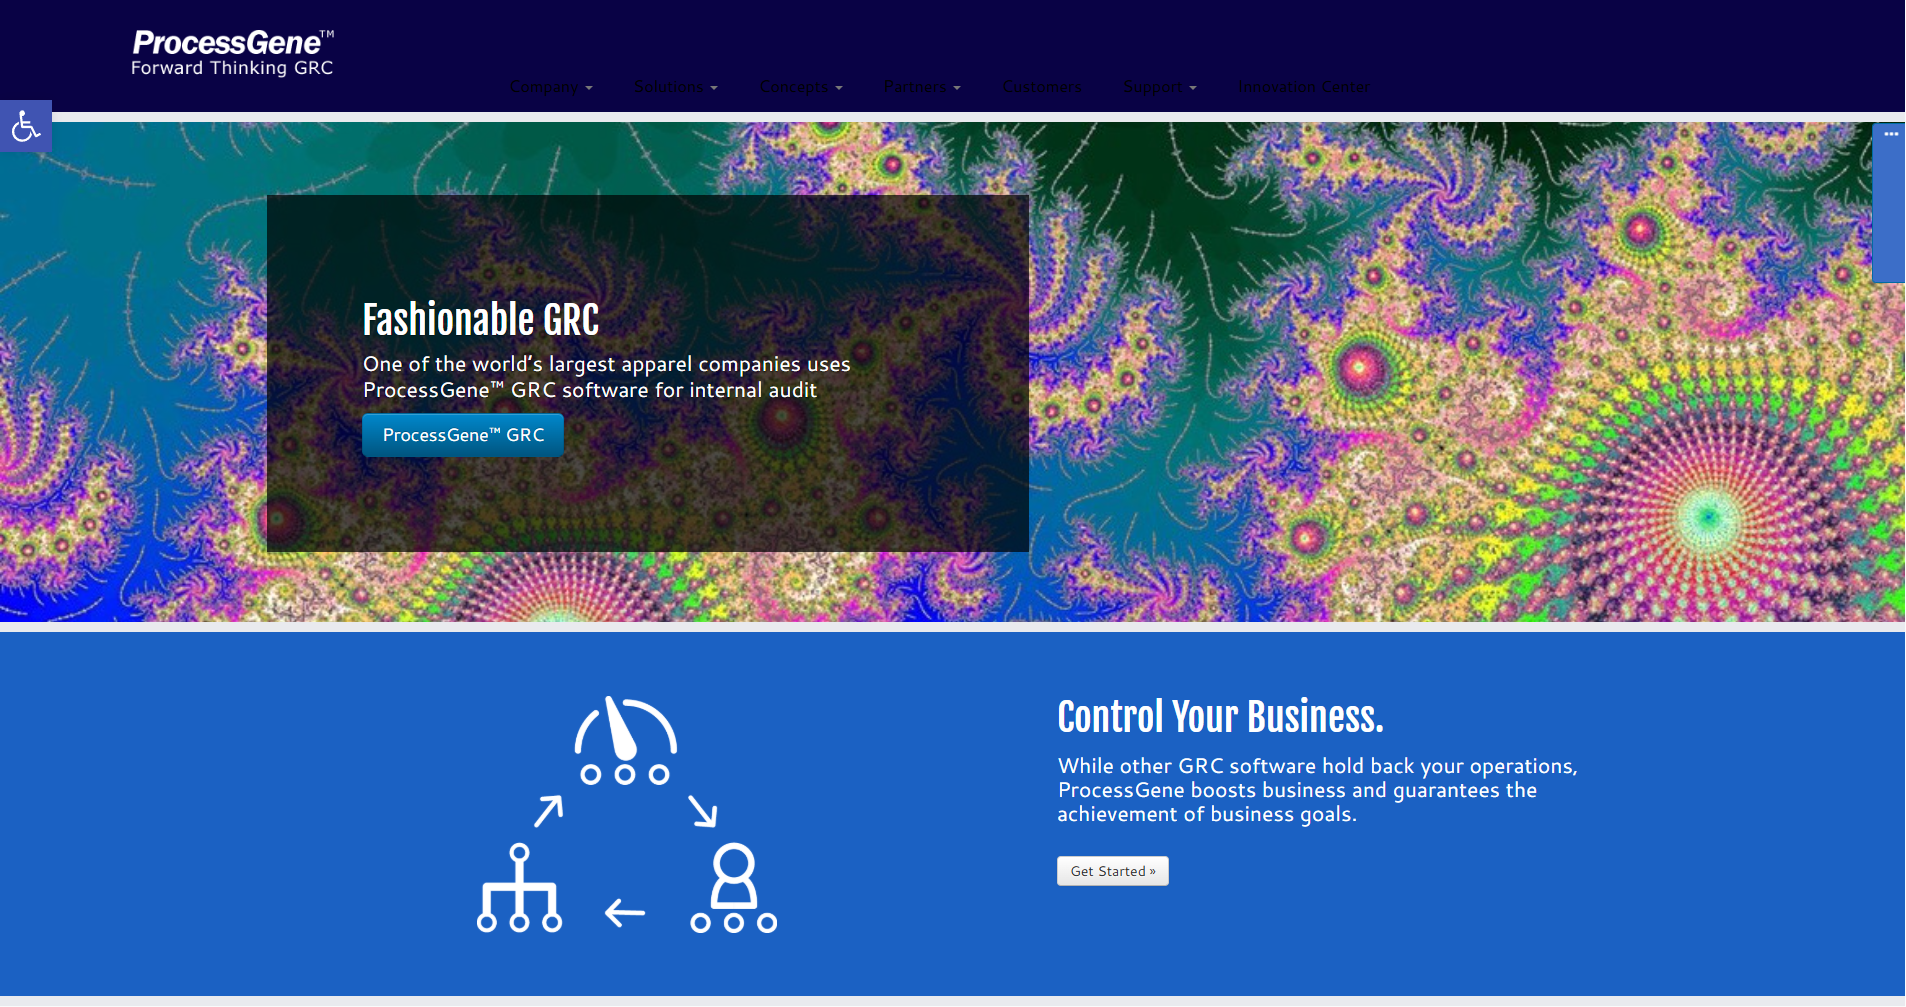
\includegraphics[width=13cm,height=8cm]{images/processgene.PNG}%
    }
    \caption{Site web ProcessGene}%
\end{figure}

\noindent\large\textbf{Comparaison des applications existantes}\normalsize
\vspace{0.3em}

\noindent Après analyse des applications existantes, il apparaît qu'il y a des points positifs et négatifs. Le Tableau 1.1 détaille une étude comparative de ces applications basée sur les fonctionnalités que nous considérons essentielles.

\begin{table}[h]
\small
\centering
\setlength{\tabcolsep}{4pt}
\caption{Tableau comparatif de l'existant}
\label{table:comparaison-verticale}
\begin{tabularx}{\textwidth}{|l|>{\centering\arraybackslash}X|>{\centering\arraybackslash}X|}
\hline
\textbf{Critère} & \textbf{AuditBoard} & \textbf{ProcessGene} \\ \hline
Gestion des audits & + & + \\ \hline
Plans d'action & + & - \\ \hline
Statistiques et tableaux de bord & + & + \\ \hline
Gestion des utilisateurs & + & - \\ \hline
Revues de direction & + & - \\ \hline
Gestion de l'historique & - & - \\ \hline
\end{tabularx}
\end{table}

\subsection{Idée émergente}

\noindent L'analyse des défis identifiés révèle l'opportunité de créer une plateforme numérique spécialisée combinant automatisation, gestion collaborative des rôles, et traçabilité complète.

Cette approche transformerait les processus manuels en workflows digitalisés structurés, adaptés aux contraintes des PME de conseil.

\subsection{Solution proposée}

\noindent Pour répondre aux défis des audits manuels, souvent lents et propices aux erreurs, nous avons conçu "Prévention Plus", une application web qui simplifie et organise la gestion des audits pour les bureaux de conseil. Cette solution permet de structurer les audits en étapes claires, de gérer les utilisateurs et leurs rôles, de suivre les plans d'action, de produire des statistiques détaillées, de gérer les revues de direction, et de conserver un historique des actions. Développée pour répondre aux besoins des PME, elle assure une traçabilité complète et le respect des normes de sécurité et de qualité.

\section{Méthodologie de travail}

\subsection{Méthodologie de travail}

\noindent Scrum [1] représente un framework organisationnel qui aide les équipes à gérer des projets complexes et évolutifs, en se concentrant sur la livraison régulière de produits à forte valeur ajoutée. Cette approche met l'accent sur la collaboration d'équipe et promeut l'amélioration progressive à travers des cycles de développement courts et répétés, visant avant tout la satisfaction des utilisateurs finaux.

La méthode Scrum s'appuie sur les principes du contrôle empirique et se base sur trois éléments fondamentaux : la visibilité complète des processus, l'évaluation continue des résultats et l'ajustement permanent des pratiques.

\begin{figure}[H]%
    \center%
{
    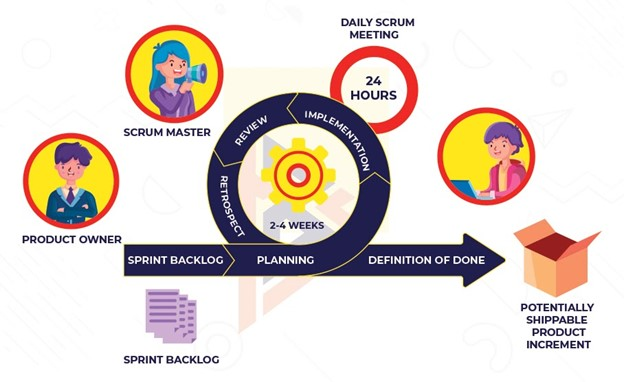
\includegraphics[width=12cm,height=6cm]{images/scrum method.jpg}%
    }
    \caption{La Méthodologie Scrum}%
\end{figure}

\subsection{Les rôles dans SCRUM}

\noindent La méthodologie SCRUM définit trois fonctions spécifiques :
\begin{itemize}
    \item \textbf{Product Owner} : Responsable qui vise à optimiser la valeur du produit généré par l'équipe de développement. Il cherche à maximiser les bénéfices commerciaux du projet. Sa mission consiste à traduire les besoins des utilisateurs et à maintenir la viabilité économique durant toute la durée du projet.

    \item \textbf{Scrum Master} : Facilitateur qui guide l'équipe dans l'application du cadre Scrum. Sa fonction principale est d'accompagner l'équipe vers une maîtrise et une application appropriées des concepts, méthodes et principes de Scrum.

    \item \textbf{Équipe de développement Scrum} : Groupe de professionnels qui construisent les éléments livrables du projet. L'équipe travaille de manière collective et s'engage à produire un incrément fonctionnel et potentiellement utilisable du produit finalisé à l'issue de chaque sprint.
\end{itemize}

\subsection{Les artefacts Scrum}

\noindent Les artefacts Scrum constituent les outils du framework Scrum qui concrétisent le travail à accomplir, comprenant trois éléments principaux :
\begin{itemize}
    \item \textbf{Product backlog} : Liste hiérarchisée et régulièrement mise à jour des tâches nécessaires pour perfectionner le produit. Il regroupe des éléments variés comme des nouvelles fonctionnalités, des exigences, des optimisations ou des résolutions de bugs, sous la supervision du Product Owner.

    \item \textbf{Sprint backlog} : Planification des objectifs visés pour le sprint en cours, ainsi que de l'incrément attendu en fin de période. Il rassemble les user stories à développer pendant le sprint accompagnées de la stratégie nécessaire pour atteindre les buts fixés.

    \item \textbf{Incrément produit} : Partie fonctionnelle du produit final, qui génère de la valeur et reste exploitable. Il vient compléter les incréments antérieurs dans la construction progressive du produit. Un sprint peut donner naissance à plusieurs incréments.
\end{itemize}

\subsection{Les réunions dans SCRUM}

\noindent Les cérémonies Scrum constituent des composants essentiels du framework Scrum qui facilitent le travail collaboratif de l'équipe et la production de fonctionnalités utiles. Voici les principales cérémonies Scrum :
\begin{itemize}
    \item \textbf{Sprint} : Période de travail intensive et limitée dans le temps nécessaire à une équipe Scrum pour accomplir un volume de tâches défini.

    \item \textbf{Planification de sprint} : Séance organisée au début de chaque sprint. L'équipe examine le backlog produit, échange sur les priorités et s'accorde sur le périmètre et les fonctionnalités qu'elle s'engage à réaliser avant la fin du sprint.

    \item \textbf{Daily Scrum} : Réunion quotidienne de 15 minutes maximum qui se tient chaque matin. Chaque membre de l'équipe s'exprime pour informer ses collègues du travail accompli la veille, des tâches prévues pour la journée et des difficultés rencontrées.

    \item \textbf{Revue de sprint} : Séance où l'équipe projet expose aux parties prenantes les différents livrables achevés. Elle permet de réaliser une démonstration pratique pour vérifier que le produit correspond aux attentes formulées par le client.

    \item \textbf{Rétrospective de sprint} : Réunion de clôture du sprint. L'équipe Scrum se rassemble pour analyser le sprint terminé, en extraire les leçons apprises et optimiser son efficacité pour la prochaine itération.
\end{itemize}

\section*{CONCLUSION}

\noindent Dans le premier chapitre, nous avons commencé par présenter le cadre général en donnant la problématique, puis nous avons décrit l'organisme d'accueil, étudié quelques exemples existants et les avons critiqués, tout en présentant la solution que nous proposons. Nous avons également exposé la méthodologie de travail adoptée pour le développement. Dans le deuxième chapitre, nous allons parler des besoins de notre projet.